% threepennygui-Hr.tex
\begin{hcarentry}[new]{threepenny-gui}
\label{threepenny-gui}
\report{Heinrich Apfelmus}%11/13
\status{active development}
\makeheader

Threepenny-gui is a framework for writing graphical user interfaces (GUI) that uses the web browser as a display. Features include:

\begin{itemize}
\item \emph{Easy installation.} Everyone has a reasonably modern web browser installed. Just install the library from hackage and you are ready to go. The library is cross-platform.
\item \emph{HTML.} You have all capabilities of HTML at your disposal when creating user interfaces. This is a blessing, but it can also be a curse, so the library includes a few layout combinators to quickly create user interfaces without the need to deal with the mess that is CSS. A small JavaScript FFI allows you to include JS client libraries.
\item \emph{Functional Reactive Programming (FRP)} promises to eliminate the spaghetti code that you usually get when using the traditional imperative style for programming user interactions. Threepenny has an FRP library built-in, but its use is completely optional. Employ FRP when it is convenient and fall back to the traditional style when you hit an impasse.
\end{itemize}

\emph{Status.}
The project is alive and kicking, version \verb`0.3.0.1` is the latest release. You can download the library from hackage and use it right away to write that cheap GUI you need for your project. Here a screenshot from the example code:

%**<img src="./chat.jpg">
%*ignore
\begin{center}
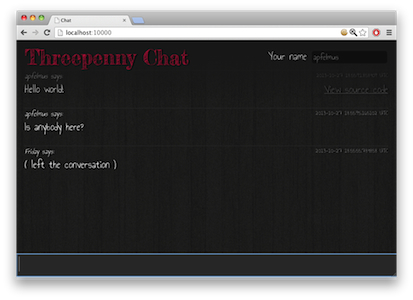
\includegraphics{html/chat.jpg}
\end{center}
%*endignore

For a collection of real world applications that use the library, have a look at the gallery on the homepage. Daniel Austin's \verb`FNIStash` program is also featured in this report \cref{FNIStash}.

\emph{Current development.}
The library is still very much in flux, significant API changes are likely in future versions. The goal is make GUI programming as simple as possible, and that just needs some experimentation.

The next version of threepenny-gui will include automatic garbage collection for HTML elements and it will (re-)introduce a \verb`UI` monad that simplifies the JavaScript FFI and supports recursive uses of FRP.

\FurtherReading
\begin{compactitem}
\item Project homepage: \url{http://haskell.org/haskellwiki/Threepenny-gui}
\item Example code: \url{https://github.com/HeinrichApfelmus/threepenny-gui#examples}
\item Application gallery: \url{http://haskell.org/haskellwiki/Threepenny-gui#Gallery}
\end{compactitem}
\end{hcarentry}
